\fullWidthTwoColumnFigureTable%
	[!t] % Placement
	{0d/figures/sc_i_uv_initial_condition.pdf} % Figure
	{fig:sc_i_uv_initial_condition} % Figure label
	{%
		The plot shows the \uv{} potential $U ( \sigma )$ (red-dashed) and its first derivative $u ( \sigma ) = \partial_\sigma U ( \sigma )$ (blue, solid) of test case I from \cref{eq:testing_scenario_non-analytic_quadaratic_asymptote}. 
		\fromFig{4}{zerod1}%
	} % Figure caption
	{%
		\renewcommand{\arraystretch}{1.15}
		\small
		\begin{tabular}{l c c c}
			\toprule
			$N$		&	$\Gamma^{(2)}$	&	$\Gamma^{(4)}$	&	$\Gamma^{(6)}$	\\
			\midrule
			$1$		&	$0.176813$		&	$0.052055$		&	$\phantom{-}0.086573$ \\
			$3$		&	$0.397354$		&	$0.140864$		&	$\phantom{-}0.224996$ \\
			$10$	&	$0.845144$		&	$0.151933$		&						$-0.069134$\\
			\bottomrule
		\end{tabular}
	} % Table content
	{tab:sc_1_n_point_functions_exact}% Table label
	{%
		Exact results for $\Gamma^{(2n)}$ of the $O(N)$ model with the \uv{} initial potential \eqref{eq:testing_scenario_non-analytic_quadaratic_asymptote} for selected $N$.
		They are obtained by a high-precision one-dimensional numerical integration of the expectation values $\langle ( \vec{\phi}^{\, 2} )^n \rangle$ from \cref{eq:ON_expectation_value} using \textit{NIntegrate} in \WAMXIIwR{}.
		Here, we present the first six digits only.
		\fromTab{I}{zerod1}%
	} % Table caption
\subsubsection{Test case I: Non-analytic initial condition}\label{subsubsec:sc1}
Consider the following \uv{} initial potential,
\begin{align}
	U ( \vec{\varphi} \vts ) =
	\begin{cases}
		- \tfrac{1}{2} \, \vec{\varphi}^{\vts 2} \, ,			&	\text{if} \quad |\vec{\varphi}| \leq 2 \, ,\\
		- 2 \, ,									&	\text{if} \quad 2 < |\vec{\varphi}| \leq 3 \, ,\\
		+ \tfrac{1}{2} \, ( \vec{\varphi}^{\vts 2} - 13 ) \, ,	&	\text{if} \quad |\vec{\varphi}|>3 \, ,
	\end{cases}	\label{eq:testing_scenario_non-analytic_quadaratic_asymptote}
\end{align}
which is plotted in \cref{fig:sc_i_uv_initial_condition}.
This initial condition for the zero-dimensional \ON{} model \dash{} in the following sometimes just referred to as \textit{test case I} \dash{} is designed this way for the following reasons:
\begin{enumerate}
	\item	All parameters of the potential $U ( \vec{\varphi} )$ are by default dimensionless and chosen to be approximately of order one, such that scales can easily be compared with each other.
	
	\item	The \uv{} potential evaluated on the mean-field $\sigma$, $U ( \sigma )$, has non-analytical points at $\sigma = 2$ and $\sigma = 3$, which correspond to discontinuities in its derivative $u ( \sigma )$.
	In the fluid-dynamical context such discontinuities present a Riemann problem and result in rarefaction waves, \cf{} \cref{subsec:hydroEuler}.
	In \qft{} and thermodynamics such discontinuities can be associated with phase 	transitions, see \MWApp{}.
	The non-analytical behavior of this potential makes commonly used techniques like the \frg{} Taylor expansion inapplicable.
	Furthermore, naive discretizations that rely on smoothness are doomed to fail.
	One has to choose numerical schemes that can handle this numerically challenging dynamics.
	
	\item	The potential is initialized in the symmetry-broken phase, with infinitely many degenerate minima at $\sigma \in ( 2, \, 3]$.
	Furthermore, the \uv{} potential is neither convex nor smooth.
	However, in the \ir{} the $O(N)$ symmetry has to be restored and there must only be one minimum at $\sigma = 0$, due to the \cmwhTheorem{}, \ie{}, in zero-dimensions $\varphi_a = \langle \phi_a \rangle = 0$, which follows directly from the integral \eqref{eq:def_corr_func_ON}.
	Furthermore, for $t \rightarrow \infty$ the potential has to be convex and smooth, see \MWApp{}.
	This non-trivial transition and complicated dynamics from the \uv{} to the \ir{} is a numerically challenging test.
	
	\item	Furthermore, we choose a potential which is asymptotically quadratic in $\sigma$.
	This is to ensure that the large-$\sigma$ \bc{} for $u ( t, \sigma )$ is fully under control and errors can be excluded, see \cref{subsec:boundary_conditions_finite_volume}. 
	This allows for a high-precision analysis of all other sources of numerical errors.
\end{enumerate}
The reference values for the exact \ir{} \ipi{} vertex functions $\Gamma^{(2n)}$ of the $O(N)$ model are calculated numerically from the \uv{} potential \eqref{eq:testing_scenario_non-analytic_quadaratic_asymptote} via the integral \eqref{eq:ON_expectation_value} using \cref{eq:on-model_relation_2pf_phi2}\nolinebreak[3]--\nolinebreak[2]\eqref{eq:on-model_relation_6pf_phi2}.
They are listed in \cref{tab:sc_1_n_point_functions_exact} for selected $N$ which are relevant for the following discussions.

In the remainder of this subsubsection we will use test case I \eqref{eq:testing_scenario_non-analytic_quadaratic_asymptote} to discuss
\begin{itemize}
	\item \customref{paragraph:ONadvDif}{Advection and diffusion in FRG flows},
	\item \customref{paragraph:ONdeltax}{Tests of the spatial resolution},
	\item \customref{paragraph:test_size_computational_domain}{Tests of the size of the computational domain},
	\item \customref{paragraph:ONRGconsistency}{Tests of the UV and IR scales}, % WARNING: do not use acronyms \uv and \ir, leads to uneven coloring of the link
\end{itemize}
in the corresponding paragraphs which are based on Secs. V.~A.1\dash{}4 of \ccite{zerod1}.

\paragraph{Advection and diffusion in \frg{} flows}\phantomsection\label{paragraph:ONadvDif}\mbox{}\\%
\subcaptionFigureOneTwo%
	[!t]% placement
	{0d/figures/sc_i_on_3_n_800_xmax_10_lambda_1e6_tir_60_rg_flow.pdf}% figA
	{%
		\caption{Snapshots of the \frg{} flow at different times ${t = 0, \, 2, \, 4, \, \ldots, \, 60}$ (integer values for $t$ were chosen for convenience and readability).}%
		\label{fig:sc_i_on_3_n_800_xmax_10_lambda_1e6_tir_60_rg_flow_2d}%
	}% caption/label (a)
	{%
		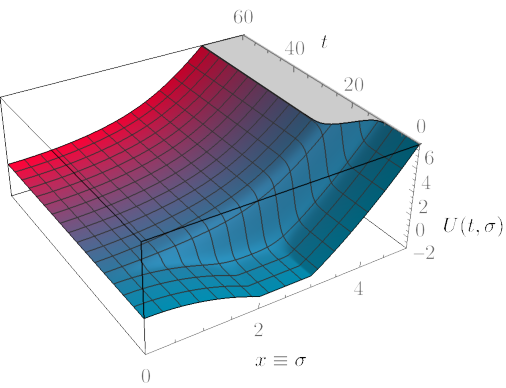
\includegraphics[width=5.5cm]{0d/figures/sc_i_on_3_n_800_xmax_10_lambda_1e6_tir_60_rg_flow_u_3d.pdf}
		\caption{Three-dimensional rendering of the flow $U(t,\sigma)$ displayed on the left \dash{} \Cref{fig:sc_i_on_3_n_800_xmax_10_lambda_1e6_tir_60_rg_flow_2d} (upper panel).}%
		\label{fig:sc_i_on_3_n_800_xmax_10_lambda_1e6_tir_60_rg_flow_u_3d}%
	}% figure/caption/label (b)
	{%
		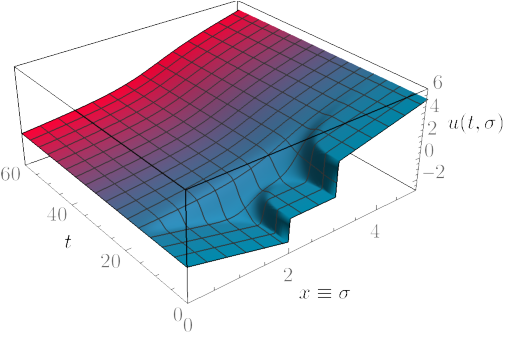
\includegraphics[width=5.5cm]{0d/figures/sc_i_on_3_n_800_xmax_10_lambda_1e6_tir_60_rg_flow_du_3d.pdf}
		\caption{Three-dimensional rendering of the flow $u(t,\sigma)$ displayed on the left \dash{} \Cref{fig:sc_i_on_3_n_800_xmax_10_lambda_1e6_tir_60_rg_flow_2d} (lower panel).}%
		\label{fig:sc_i_on_3_n_800_xmax_10_lambda_1e6_tir_60_rg_flow_du_3d}%
	}% figure/caption/label (c)
	{%
	The \frg{} flow of the effective potential $U ( t, \sigma )$ \dash{} upper panel/figure on the left~\subref{fig:sc_i_on_3_n_800_xmax_10_lambda_1e6_tir_60_rg_flow_2d} and on the right~\subref{fig:sc_i_on_3_n_800_xmax_10_lambda_1e6_tir_60_rg_flow_u_3d} \dash{} and its derivative $u ( t , \sigma ) = \partial_\sigma U ( t , \sigma )$ \dash{} lower panel/figure on the left~\subref{fig:sc_i_on_3_n_800_xmax_10_lambda_1e6_tir_60_rg_flow_2d} and on the right~\subref{fig:sc_i_on_3_n_800_xmax_10_lambda_1e6_tir_60_rg_flow_du_3d} \dash{} for the zero-dimensional $O ( 3 )$ model with initial condition \eqref{eq:testing_scenario_non-analytic_quadaratic_asymptote}. 
	The blue curves correspond to the \uv{} and the red curves to the \ir{}.
	We used the exponential regulator~\eqref{eq:exponential_regulator} with \uv{} scale $\Lambda = 10^6$.
	For the sake of readability, the plots do not show the region ${x \in[5,10]}$, because the tiny differences between $u ( t , \sigma )$ and $u ( 0 , \sigma )$ are not visible in this region and vanish for large $x = \sigma$ anyhow.
	\fromFigs{5, 6, and 7}{zerod1}%
	}% caption
	{fig:sc_i_on_3_n_800_xmax_10_lambda_1e6_tir_60_rg_flow}% label
We start our analysis with a general discussion of the \frg{} flow with \ic{} \eqref{eq:testing_scenario_non-analytic_quadaratic_asymptote}.
To this end, we fix $O(N = 3)$ to include both diffusive and advective contributions via the radial \sigmaMode{} and two pions. For $N = 3$ the number of pions is reasonably small and the (diffusive) effects of the \sigmaMode{} remain visible.
Furthermore, we choose $[ 0, x_\mathrm{max} = 10 ]$ as the spatial computational domain with $n=800$ volume cells and use the \ktScheme{} from \cref{subsec:hydroKT} for spatial discretization.
The initial cell averages $\bar{u}_i ( t = 0 )$ are computed by exact averaging\footnote{%
	Using the exact averages for $\bar{u}_i(t=0)$ has proven advantageous in terms of achievable numerical precision in the \ir{} compared to taking the mid-point values of the exact derivative of ${ \bar{u}_i ( t = 0 ) = \partial_\sigma U ( \sigma ) |_{\sigma = \sigma_i} }$ when considering non-analytic \ics{} like \cref{eq:testing_scenario_non-analytic_quadaratic_asymptote} or \eqref{eq:testing_scenario_4}.%
} 
\begin{align}
	\bar{u}_i ( t = 0 ) = \frac{1}{\Delta \sigma} \, \big[ U \big( \sigma_{i + \frac{1}{2}} \big) - U \big( \sigma_{i - \frac{1}{2}} \big) \big] ,
\end{align}
using the \uv{} \ic{} \eqref{eq:testing_scenario_non-analytic_quadaratic_asymptote}.
We use linear extrapolation \eqref{eq:BClinExt} as spatial \bc{} at $x_\mathrm{max}$ as discussed in \cref{paragraph:BCinf}.
The \uv{} scale is set to $\Lambda = 10^6$ at $t = 0$. 
Time evolution of the semi-discrete \kt{} \ode{} system is performed with \textit{NDSolve} of \WAMXIIwR{} with a \textit{PrecisionGoal} and \textit{AccuracyGoal} of 10 and stopped in the \ir{} at $r ( t_\mathrm{IR} = 60 ) \approx 10^{-20}$ using the exponential regulator shape function \eqref{eq:exponential_regulator}.
Time-stepping has not been a focus of our work and we refer the interested reader to the excellent \ccite{Ihssen:2023qaq} discussing the issue in the context of \frg{} in detail.
We find that this choice of parameters suffices to produce decent results, as discussed in the following.
There, we quantitatively analyze sources and severity of possible errors related to those (numerical) parameters.

We first provide qualitative results of our numerical methods in \cref{fig:sc_i_on_3_n_800_xmax_10_lambda_1e6_tir_60_rg_flow}, where we show the \frg{} flow of the effective potential $U ( t, \sigma )$ and its derivative $u ( t, \sigma ) = \partial_\sigma U ( t, \sigma )$ from the \uv{} (blue) to the \ir{} (red).
In the beginning, \ie{}, in the \uv{}, the system is in the broken phase. 
This changes only marginally until $t \approx 7$, which indicates that the \uv{} scale is chosen sufficiently large with $\Lambda = 10^6$.
When $r(t)$ reaches the scales of the model at $t \smallergtrsim 11$ most of the dynamics takes place (symmetry restoration) and $u ( t, \sigma )$ changes rapidly and drastically until it freezes out in the \ir{}.
In the \ir{} the system is in the restored phase as expected \apriori{}.
After $t \approx 26$ the potential does not change anymore, which indicates that one has reached a sufficiently small \ir{} scale to stop the integration.
We render this statement more precise in the following \cref{paragraph:ONRGconsistency}.
Note that the evolution in $t$ is logarithmic and corresponds to a change in scale over $25$ orders of magnitude.
At first glance this range sounds excessive, but its necessity is explained in detail in \cref{paragraph:ONRGconsistency}.

During the \frg{} evolution one observes that diffusive processes smear out the discontinuities at the non-analytic points at $\sigma = 2$ and $\sigma = 3$.
We also find that the diffusion acts in both directions \dash{} towards larger and smaller values of $\sigma$ \dash{} as expected from our discussion in \cref{subsubsec:conservative_form}. 
Nevertheless, the diffusive effects do not reach the computational boundary, which is outside the plot range at $\sigma_\mathrm{max} = 10$.
This suggests that $\sigma_\mathrm{max} = 10$ is sufficiently large.
Additionally, we observe a propagation of the conserved quantity $u$ towards smaller values of $\sigma$ via advection. 
Close to the initial discontinuities these advective processes can be interpreted as rarefaction waves. 
In a more pictorial language, the advection and diffusion ``fill up the pit'' in $u ( t, \sigma )$ at small values of $\sigma$ by moving more and more of the quantity $u$ from larger values of $\sigma$ to smaller $\sigma$ (via advection and diffusion) as well as from small negative $\sigma$ to small positive $\sigma$ (via diffusion).
Eventually the symmetry is restored and $u ( t, \sigma )$ is smoothed towards the \ir{} by diffusion. 
Furthermore, the conserved quantity $u$ does not ``pile up'' at $\sigma = 0$ after symmetry restoration, because at negative $\sigma$ exactly the opposite dynamics happens, due to the \ZII{} antisymmetry of $u ( t, \sigma )$, which is encoded in the \bc{} at $\sigma = 0$, see \cref{subsec:boundary_conditions_finite_volume}.
The differences between advective and diffusive contributions become apparent when comparing the same system for different $N$, \cf{} \cref{fig:sc_i_on_1_10_100_n_800_xmax_10_lambda_1e6_tir_60_rg_flow} and the surrounding discussion.

From a numerical perspective, the \ktScheme{} is able to handle the highly non-linear dynamics, including the non-analyticities in $u ( t, \sigma )$, without any spurious oscillatory behavior (under-/over-shooting) and allows for a stable $t$ integration to extremely small \ir{} scales.

For the sake of completeness and illustrative purposes, we also provide the \frg{} flow of the integral of $u ( t, \sigma )$, \ie{}, the effective potential $U ( t, \sigma )$, in \cref{fig:sc_i_on_3_n_800_xmax_10_lambda_1e6_tir_60_rg_flow_2d} (upper panel) and \cref{fig:sc_i_on_3_n_800_xmax_10_lambda_1e6_tir_60_rg_flow_u_3d}.
Here, the integration constant was set to zero\footnote{%
	$U ( t, 0 ) = 0$ is dictated by our choice of normalization for the zero-point function(s), see \cref{eq:normalization}.
} and the integration was performed via Riemann summation\footnote{%
	At this point we should mention that numerical results for $U ( t, \sigma )$ via Riemann summation should be treated with great caution: Numerical errors in the cell averages $\bar{u} ( t, x_j )$ which arise from the numerical \frg{} flow can accumulate during integration (here summation) along $\sigma = x$.
	More precise quadrature methods should be used if precise, quantitative values for $U ( t, \sigma )$ are needed.
} of the discrete cell averages,
	\begin{align}
		U ( t, x_i ) = \Delta x \sum_{j = 0}^{i} \frac{\bar{u} ( t, x_j )}{( 1 + \delta_{j, 0} + \delta_{j, i} )} \, .	\label{eq:riemann_sum}
	\end{align}
\Cref{fig:sc_i_on_3_n_800_xmax_10_lambda_1e6_tir_60_rg_flow_u_3d} perfectly illustrates the restoration of the $O(3)$ symmetry of the potential $U ( t, \sigma )$ during the \frg{} flow via ``vaporization'' of the infinitely many minima.
Nevertheless, we find that it is hardly possible to intuitively understand the contributions of the radial \sigmaMode{} and the pions to the \frg{} flow on the level of $U ( t, \sigma )$ only.
This complements the discussion in \cref{subsubsec:conservative_form} and lends support to our claim that the fluid-dynamical interpretation of the \frg{} flow in terms of $u ( t, \sigma )$ is superior to the canonical formulation in terms of $U ( t, \sigma )$ commonly used in the \frg{} literature.

\WarningFilter{latex}{Text page}
\fullWidthTwoColumnFigures%
	[!t] % Placement
	{%
		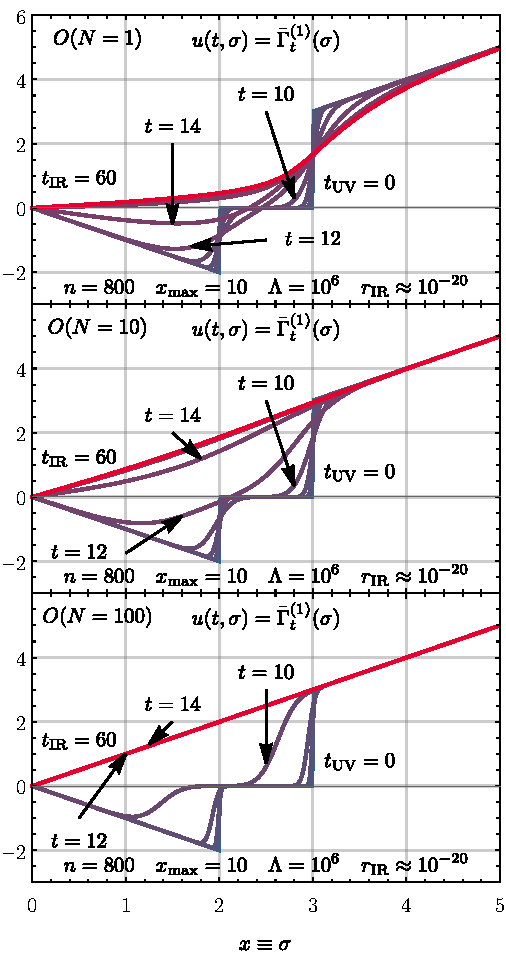
\includegraphics[width=\subcaptionFigureWidth-0.2cm]{0d/figures/sc_i_on_1_10_100_n_800_xmax_10_lambda_1e6_tir_60_rg_flow.pdf} % left figure
		\captionsetup{width=\subcaptionFigureWidth}%
		\caption{%
			The \frg{} flow of the derivative of the effective potential $u ( t , \sigma ) = \partial_\sigma U ( t, \sigma )$ for the zero-dimensional $O(N)$ model for $N = 1, \, 10, \, 100$ with \ic{} \eqref{eq:testing_scenario_non-analytic_quadaratic_asymptote}.
			All other parameters are identical to those in \cref{fig:sc_i_on_3_n_800_xmax_10_lambda_1e6_tir_60_rg_flow}.
			\fromFig{8}{zerod1}
		}
		\label{fig:sc_i_on_1_10_100_n_800_xmax_10_lambda_1e6_tir_60_rg_flow}
	}
	{\fullWidthTwoColumnFigureSpacing}
	{%
		\vspace{.065cm}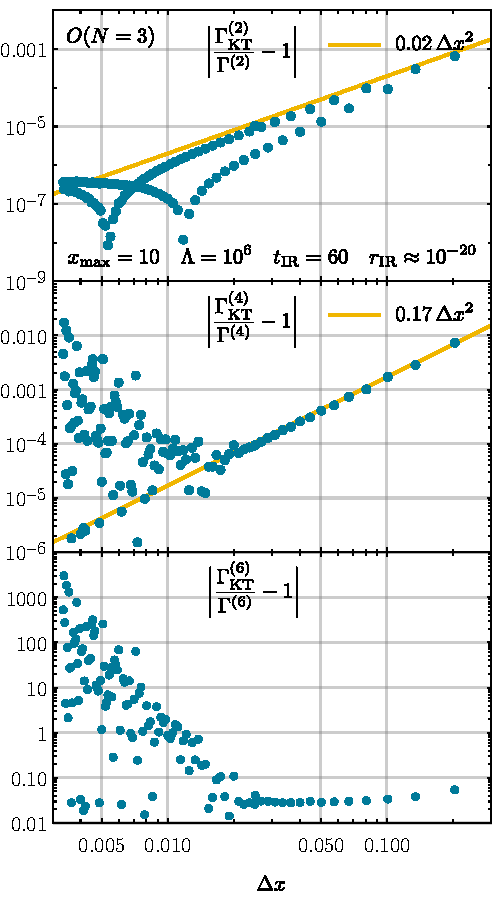
\includegraphics[width=\subcaptionFigureWidth+0.2cm]{0d/figures/sc_i_on_3_xmax_10_lambda_1e6_tir_60_deltax_scaling.pdf} % Right figure
		\captionsetup{width=\subcaptionFigureWidth}%
		\caption{%
			The relative error of the numerical results (blue dots) from the \kt{} scheme for the \ipi{} \nptFunctions{} $\Gamma^{(2n)}$ for $n = 1, 2, 3$ as a function of $\Delta x$ with \ic{} \eqref{eq:testing_scenario_non-analytic_quadaratic_asymptote}.
			The numerical derivatives at $\sigma = 0$ of $u(t_\mathrm{IR}=60, \sigma)$ were calculated via the second-order accurate central schemes \eqref{eq:derivative_1_central_error_2}, \eqref{eq:derivative_3_central_error_2}, and \eqref{eq:derivative_5_central_error_2}.
			The plot was produced with $x_\mathrm{max} = 10$, but could have been calculated for any sufficiently large $x_\mathrm{max}$.
			We used the exponential regulator~\eqref{eq:exponential_regulator} with \uv{} scale $\Lambda = 10^6$.
			The yellow straight lines $\propto \Delta x^2$ are for optical guidance.
			\fromFig{9}{zerod1}%
		}%
		\label{fig:sc_i_on_3_xmax_10_lambda_1e6_tir_60_deltax_scaling}
		\vspace{1cm}
	}%
\WarningFilter*{latex}{Text page}
Before discussing quantitative results and sources of (numerical) errors in \frg{} flows, we briefly return to the interpretation of the radial \sigmaMode{} as diffusion and the interpretation of the pions as advection in the \frg{} flow along the field space direction.
To this end, we discuss \frg{} flows for the same \uv{} initial potential \eqref{eq:testing_scenario_non-analytic_quadaratic_asymptote} as before, but for different $N$.
This  corresponds to a different number of pions in the flow and different advection velocities \eqref{eq:advection_velocity}.
All other parameters remain unchanged.
In addition to the $N = 3$ case in \cref{fig:sc_i_on_3_n_800_xmax_10_lambda_1e6_tir_60_rg_flow}, we provide the \frg{} flows of $u ( t, \sigma )$ for $N = 1, 10, 100$ in \cref{fig:sc_i_on_1_10_100_n_800_xmax_10_lambda_1e6_tir_60_rg_flow}.
The figure again demonstrates on a qualitative level that the \sigmaMode{} enters the \frg{} as diffusion, while pions enter as advection: Increasing the number of pions the problem becomes more advection-driven exhibiting more pronounced waves and faster propagation.
This can be seen by comparing the plots at equal \rgtimes{}.
For $N = 1$, the problem reduces to the pure diffusion equation \eqref{eq:pde_gamma}, where the dynamics is slowest and the diffusion propagates the fluid from negative $\sigma$ to small positive $\sigma$ close to $\sigma = 0$.
Furthermore, one observes stronger smearing of the discontinuities at $\sigma = 2$ and $\sigma = 3$.
The $N = 100$ case is extremely advection-dominated.
In the fluid-dynamical language, this corresponds to a complete suppression of diffusion, which is clearly observed from the fast propagation of the rarefaction waves and almost negligible smoothing of the discontinuities at $\sigma = 2$ and $\sigma = 3$.
We will discuss the qualitative and quantitative differences between \frg{} flows at small $N$ with flows large and even infinite $N$ in \cref{subsec:0dLargeN}.

\paragraph{Tests of the spatial resolution}\phantomsection\label{paragraph:ONdeltax}\mbox{}\\%
This paragraph is dedicated to quantifying numerical errors in the \frg{} flow arising from the finite spatial resolution $\Delta x\equiv \Delta \sigma$ of the cells in the \ktScheme{}.
Any spatial discretization comes with a discretization error.
The \ktScheme{}, which is used throughout this thesis, is formally of second-order accuracy in $\Delta x$ when employing the numerical fluxes of \cref{eq:FVKTO2} with the five-point stencil \eqref{eq:kt_stencil}.
Therefore, the numerical errors arising from the spatial discretization should scale with $\Delta x^2$ when $\Delta x$ is decreased.

As test values (observables) we use the modulus of the relative errors of the \ipi{} \nptFunctions{} $\Gamma^{(2n)}$ for $n = 1, 2, 3$,
\begin{align}
	\bigg| \frac{\Gamma^{(2n)}_\mathrm{KT}}{\Gamma^{(2n)}} - 1 \bigg| \, ,	\label{eq:relative_errors_gamma_2n}
\end{align}
where $\Gamma^{(2n)}_\mathrm{KT}$ is calculated from the \frg{} (via the \ktScheme{}) and $\Gamma^{(2n)}$ from the integral, see \cref{tab:sc_1_n_point_functions_exact}.
In order to determine how much of the relative numerical error~\eqref{eq:relative_errors_gamma_2n} is directly related to the spatial discretization, we have to optimize all other parameters of the computation in order to reduce other sources of errors.
We basically choose the same parameter set \dash{} \viz{} $\Lambda = 10^6$, $x_\mathrm{max} = 10$ and $t_\mathrm{IR} = 60$ \dash{} and \uv{} \ic{} \eqref{eq:testing_scenario_non-analytic_quadaratic_asymptote} which was also used for the qualitative analysis in the previous paragraph and only vary the number of cells $n$ to change the resolution $\Delta x$.
\WlogA{} we keep $N=3$.

Before we embark on our discussion, we remark that the spatial-discretization error enters the relative errors~\eqref{eq:relative_errors_gamma_2n} in a twofold way: 
\begin{enumerate}
	\item	There is the discretization error which comes from the \ktScheme{} during the \frg{} time integration.
	This error shows up directly in the \ir{} values $u ( t_\mathrm{IR}, x_i )$ and should scale according to $\Delta x^2$ for the chosen second-order \ktScheme{}.

	\item	There is a discretization error which is related to the extraction of the \ipi{} \nptFunctions{} from the discrete $\bar{u} ( t_\mathrm{IR}, x_i )$. 
	They have to be calculated at the physical point (the minimum at $x = \sigma = 0$) via numerical differentiation, which also comes with a discretization error.
	The latter is also related to the spatial resolution $\Delta x$.
	In general (especially in higher-dimensional models) it is not clear whether these numerical derivatives at the physical point are always well-defined.
	We argued before that $u ( t, \sigma )$ might exhibit non-analytical behavior also at the physical point in the \ir{}, \cf{}\ \ccite{Grossi:2019urj,Grossi:2021ksl,Borchardt:2016pif,Stoll:2021ori}, such that a naive numerical differentiation is not allowed in general.
	In the special case of zero-dimensional \qfts{}, we proved in \MWApp{} that the \ir{} effective action and the \ir{} potential $U ( t \rightarrow \infty, \vec{\varphi}\, )$ are smooth, which also translates to $u ( t \rightarrow \infty, \sigma )$, such that numerical differentiation (\eg{}, via finite-difference approximations) is well-defined.
\end{enumerate}
However, even though finite-difference formulas are reliable approximations for derivatives of a smooth function and have a well-defined truncation-error scaling in powers of $\Delta x$, there remains a well-known subtlety: While decreasing the resolution $\Delta x$, one eventually will reach a point where the error starts increasing again contrary to the formal truncation-error scaling. 
This is related to the ill-conditioned nature of finite-difference formulas and to explicit rounding errors in floating-point arithmetic, which increase the error of the numerical derivative below a certain $\Delta x$, see, \eg{}, Chap.~5.7 of \ccite{PresTeukVettFlan92}.
Related spurious cancellations occur if the discrete data of a smooth function include some sort of noise.
In our case this ``noise'' is directly related to the spatial-discretization errors from the \ktScheme{} and the errors from \rgtime{} integration using numerical \ode{} solvers.
These errors might be tiny, but can easily inflate the errors of the numerical derivatives, especially for higher-order derivatives.

In conclusion, while decreasing $\Delta x$, we expect that long before the relative errors from the \ktScheme{} start increasing again (because the \ktScheme{} begins operating close to machine precision or because the error of the time stepping becomes relevant) the relative errors \eqref{eq:relative_errors_gamma_2n} start increasing due to the numerical differentiation of slightly ``noisy data''. 
This phenomenon is expected to set in at larger $\Delta x$ for approximations for higher-order derivatives and long before the formal error scaling of the \ktScheme{} is no longer valid.

Our explicit results for the scaling of the relative errors with decreasing spatial resolution are presented in \cref{fig:sc_i_on_3_xmax_10_lambda_1e6_tir_60_deltax_scaling}, where we show the relative errors \eqref{eq:relative_errors_gamma_2n} for the \hbox{two-}, \hbox{four-}, and six-point functions in a double-logarithmic plot over $\Delta x$.
For $\Gamma^{(2)}$ and $\Gamma^{(4)}$ we find that the corresponding relative errors scale with $\Delta x^2$ (or even slightly better) as expected from the error scaling of the \ktScheme{} as well as the error scaling of the finite-difference stencils~\eqref{eq:derivative_1_central_error_2} and \eqref{eq:derivative_3_central_error_2}.
We observe two groups of points for $\Gamma^{(2)}$ (upper panel of \cref{fig:sc_i_on_3_xmax_10_lambda_1e6_tir_60_deltax_scaling}), which are related to discretization errors of the discontinuous \ic{} \eqref{eq:testing_scenario_non-analytic_quadaratic_asymptote} at $x=2$ and $x=3$. 
The error scaling of $0.02\, \Delta x^2$ for $\Gamma^{(2)}$ is a conservative estimate for the observed errors, which are actually lower for $\Delta x \smallergtrsim 0.005$. 
For $\Delta x \smallerlesssim 0.005$ we observe deviations from the conservative estimate for the error scaling of $\Gamma^{(2)}$ related to other error sources.
In the middle panel of \cref{fig:sc_i_on_3_xmax_10_lambda_1e6_tir_60_deltax_scaling}, we clearly see that there is an optimal minimal $\Delta x \approx 0.02$ where the correct formal scaling of the numerical derivative breaks down and the relative error of $\Gamma^{(4)}$ increases again for smaller $\Delta x$.
We can be sure that this breakdown of the error scaling is related to the numerical differentiation and not the \ktScheme{} because we observe scaling with at least $\Delta x^2$ for $\Gamma^{(2)}$ in the upper panel of \cref{fig:sc_i_on_3_xmax_10_lambda_1e6_tir_60_deltax_scaling} well below $\Delta x \approx 0.02$.
This is expected for lower-order numerical derivatives.
Furthermore, we find that for $\Gamma^{(6)}$ (lower panel of \cref{fig:sc_i_on_3_xmax_10_lambda_1e6_tir_60_deltax_scaling}) the order of the numerical derivative is already too large, such that the theoretical error scaling of the \ktScheme{} cannot be seen at all and is completely obscured by the errors from the numerical differentiation of $\bar{u} ( t_\mathrm{IR}, x_i )$.

We conclude that the \ktScheme{} is perfectly suited for the spatial discretization of the \frg{} flow equation for $u ( t, \sigma )$ and shows correct scaling with decreasing spatial resolution $\Delta x$. 
This is also confirmed by tests with different \ics{}, see, \eg{}, \cref{fig:sc_ii_n_on_4_xmax_10_lambda_1e12_tir_60_deltax_scaling}.

In addition, we actually found that a more severe problem is the correct extraction of physical observables from the \ir{} values $\bar{u} ( t_\mathrm{IR}, x_i )$, which are usually related to derivatives of $u ( t_\mathrm{IR}, \sigma )$.
We predict that this problem might even become more severe in higher dimensions, were the \ir{} potential is no longer guaranteed to be smooth.
We therefore suggest to search for better ways of calculating those derivatives as well as for careful analysis tools for numerically calculated \ipi{} \nptFunctions{} in the vicinity of non-analyticities in general.
However, this is beyond the scope of the present work.

We remark that our numerical findings indicate that \dash{} independent of the specific numerical discretization scheme \dash{} the number of grid points or expansion coefficients might have been chosen too small in previous \frg{} studies in literature to obtain a decent resolution.
However, other works, \cf{} \ccite{Pelaez:2015nsa,Caillol:2012zz,Pangon:2009pj,Pangon:2010uf,Borchardt:2015rxa,Borchardt:2016pif}, which also discuss the limitations of their numerical schemes in detail, have used a rather large number of discretization points \dash{} in some cases to compensate the demand for continuity of the specific schemes.

In the following we will mostly use a spatial resolution of 
	\begin{align}
		\Delta x = \frac{x_\mathrm{max}}{n - 1} \simeq 0.025 \, ,
	\end{align}
where we can trust the results for the two- and four-point functions.
The relative errors for the six-point function will only be plotted for the sake of completeness, but cannot be included in any reasonable quantitative analysis of other sources of (numerical) errors in \frg{} flow equations although they are still at a reasonably small level of $\sim 5\%$ at $\Delta x \simeq 0.025$.

\paragraph{Tests of the size of the computational domain}\phantomsection\label{paragraph:test_size_computational_domain}\mbox{}\\%
\fullWidthTwoColumnSubFigures%
	[!t]% Placement
	{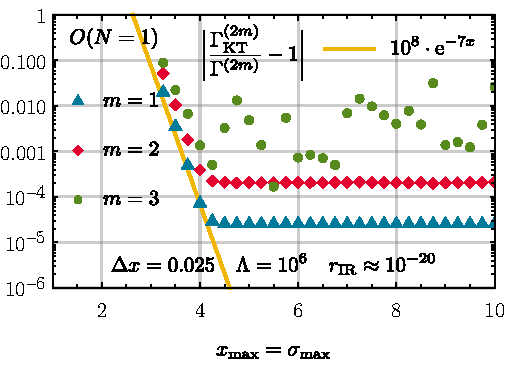
\includegraphics[width=\subcaptionFigureWidth]{0d/figures/sc_i_on_1_deltax_25e-3_lambda_1e6_tir_60_errors_xmax.pdf}}% Left figure (dummy index a)
	{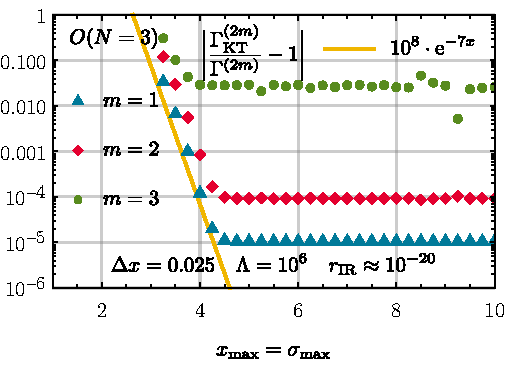
\includegraphics[width=\subcaptionFigureWidth]{0d/figures/sc_i_on_3_deltax_25e-3_lambda_1e6_tir_60_errors_xmax.pdf}}% Right figure (dummy index b)
	[fig:sc_i_on_1_deltax_25e-3_lambda_1e6_tir_60_errors_xmax,fig:sc_i_on_3_deltax_25e-3_lambda_1e6_tir_60_errors_xmax] %Labels
	{%
		The relative error for $\Gamma^{(2m)}$ for $m = 1, 2, 3$ for the \uv{} potential \eqref{eq:testing_scenario_non-analytic_quadaratic_asymptote} of the \ONn{1} model on the left \subref{fig:sc_i_on_1_deltax_25e-3_lambda_1e6_tir_60_errors_xmax} and of the \ONn{3} model on the right \subref{fig:sc_i_on_3_deltax_25e-3_lambda_1e6_tir_60_errors_xmax} as a function of $x_\mathrm{max}$, while keeping the cell size constant, $\Delta x = 0.025$. $\Gamma^{(2m)}$ are computed from the discrete values of the derivative of the \ir{} potential $u ( t_\mathrm{IR} = 60, \sigma )$ via the second-order accurate central finite-difference stencils~\eqref{eq:derivative_1_central_error_2}, \eqref{eq:derivative_3_central_error_2}, and \eqref{eq:derivative_5_central_error_2} at $\sigma = 0$.
		We use the exponential regulator~\eqref{eq:exponential_regulator} with \uv{} scale $\Lambda = 10^6$.
		The yellow straight line $\propto\exp{-7x_\mathrm{max}}$ is for optical guidance.
		\fromFigs{10 and 11}{zerod1}%
	}% Caption
	{fig:sc_i_on_deltax_25e-3_lambda_1e6_tir_60_errors_xmax}% Label
In this paragraph, we discuss the influence of the size of the computational domain $[ 0, \sigma_\mathrm{max} ]$ on the relative errors of the \ir{} observables \eqref{eq:relative_errors_gamma_2n}.
As discussed in \cref{subsec:boundary_conditions_finite_volume}, we expect that, if the spatial \bcs{} are not implemented with great caution and the computational domain is too small, one cannot trust the results from the numerical integration of the \frg{} flow.
If the computational domain is too small, we expect large errors, because the \bcs{} at $\sigma_\mathrm{max}$ are no longer valid due to wrong extrapolation to the ghost cells and consequently wrongly estimated influx.

In the case with \uv{} \ic{} \eqref{eq:testing_scenario_non-analytic_quadaratic_asymptote}, the \bc{} at $\sigma_\mathrm{max}$ is implemented as a linear extrapolation \eqref{eq:BClinExt} of $u ( t, \sigma )$ to the two ghost cells of the \ktScheme{} to mimic the asymptotic behavior of $u ( t, \sigma )$. 
As long as $\sigma_\mathrm{max}$ is sufficiently large, we expect only tiny deviations of $u ( t, \sigma )$ from its initial \uv{} value $u ( t_\mathrm{UV} = 0, \sigma )$ around $\sigma_\mathrm{max}$.
However, if $\sigma_\mathrm{max}$ is too small and approaches the model scales, we expect the diffusive effects to reach the boundary of the computational domain, such that a linear extrapolation is no longer a good approximation in order to determine the spatial \bc{}.

To this end, we test the scaling of the relative errors \eqref{eq:relative_errors_gamma_2n} with decreasing computational domain size $x_\mathrm{max} = \sigma_\mathrm{max}$ for $N = 1$ (purely diffusive) and $N = 3$. 
The results and (numerical) parameters are shown in \cref{fig:sc_i_on_deltax_25e-3_lambda_1e6_tir_60_errors_xmax}.
In both cases ($N=1$ and $N=3$ in \cref{fig:sc_i_on_1_deltax_25e-3_lambda_1e6_tir_60_errors_xmax,fig:sc_i_on_3_deltax_25e-3_lambda_1e6_tir_60_errors_xmax} respectively) we find that the relative errors are independent of $\sigma_\mathrm{max}$ for sufficiently large $\sigma_\mathrm{max}$.
However, if the spatial cutoff $\sigma_\mathrm{max}$ is approaching the model scales (here the discontinuity in $u ( t_\mathrm{UV} = 0, \sigma )$ at $\sigma = 3$, see \cref{fig:sc_i_uv_initial_condition}) the relative errors for $\Gamma^{(2)}$ and $\Gamma^{(4)}$ start rising exponentially.

Contrary to our expectations, the results for $N = 1$ and $N = 3$ are very similar and the exponential rise of the relative errors sets in at a similar $\sigma_\mathrm{max}\approx 4.2$.
\Apriori{} we expected that for the purely diffusive scenario with $N = 1$, the diffusive effects arising from the large gradients at $\sigma = 3$ might have more time to reach and influence the shape of $u ( t, \sigma )$ at larger values of $\sigma$, which does not seem to be the case.
Our employed monitors for numerical errors \dash{} the \ipi{} \nptFunctions{} in the \ir{} computed at $\sigma=0$ and $t=0$ \dash{} are rather intensive to such changes.
A possible explanation is the fact that observable errors from the boundary at $\sigma_\mathrm{max}$ propagate into the computational domain at a finite speed\footnote{
	In the context of ``infinite propagation speeds'' in parabolic \pdes{}, \cf{} the discussion and corresponding footnote~\ref{footnote:HEinf} in \cref{subsec:hydroDiffusion}, we refer here to the fact that observable changes on the relevant scales of the problem travel with apparently finite speed independent from some formal instantaneous, infinitesimal (exponentially decaying) changes.% 
}, which is rather low in the purely diffusive case and in general small at large~$\sigma$, and thus do not influence the physical point at $t=0$ and $\sigma=0$. 

Nevertheless, we conclude from \cref{fig:sc_i_on_1_deltax_25e-3_lambda_1e6_tir_60_errors_xmax,fig:sc_i_on_3_deltax_25e-3_lambda_1e6_tir_60_errors_xmax} that it is extremely important to use sufficiently large computational domains to minimize numerical errors in field-dependent \frg{} flows. 
This implies that $\sigma_\mathrm{max}$ should be chosen much larger than all relevant scales of the model.

\fullWidthTwoColumnSubFigures
	[!t] % Placement
	{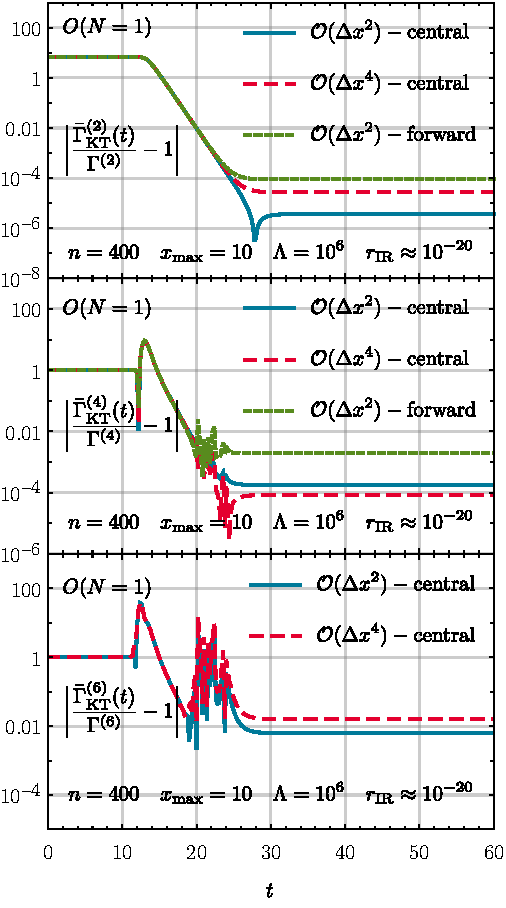
\includegraphics[width=\subcaptionFigureWidth]{0d/figures/sc_i_on_1_n_400_xmax_10_lambda_1e6_tir_60_flow_errors.pdf}} % left figure (dummy index a)
	{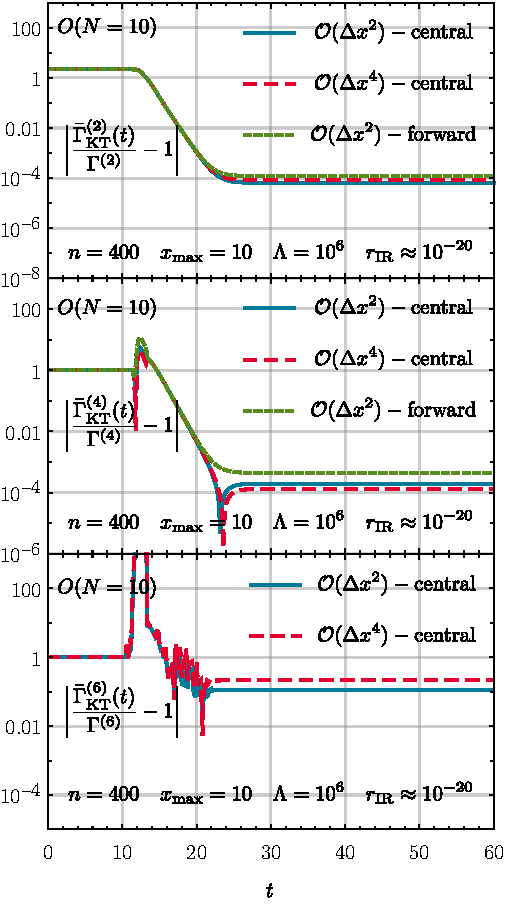
\includegraphics[width=\subcaptionFigureWidth]{0d/figures/sc_i_on_10_n_400_xmax_10_lambda_1e6_tir_60_flow_errors.pdf}} % Right figure (dummy index b)
	[fig:sc_i_on_1_n_400_xmax_10_lambda_1e6_tir_60_flow_errors,fig:sc_i_on_10_n_400_xmax_10_lambda_1e6_tir_60_flow_errors] %Labels
	{%
		The relative error for $\Gamma^{(2m)}$, for $m = 1, 2, 3$, calculated with the \kt{} scheme as a function of the \rgtime{} $t$ for the \ONn{1} model on the left~\subref{fig:sc_i_on_1_n_400_xmax_10_lambda_1e6_tir_60_flow_errors} and of the \ONn{10} model on the right~\subref{fig:sc_i_on_10_n_400_xmax_10_lambda_1e6_tir_60_flow_errors}.
		The \uv{} initial potential is given by \cref{eq:testing_scenario_non-analytic_quadaratic_asymptote}. 
		We use the exponential regulator~\eqref{eq:exponential_regulator} with \uv{} scale $\Lambda = 10^6$. 
		The computational grid has $n=400$ cells and $\sigma_\mathrm{max} = x_\mathrm{max} = 10$. $\Gamma^{(2m)}$ are extracted from $u ( t_\mathrm{IR} = 60, \sigma )$ via the finite-difference stencils \eqref{eq:derivative_1_central_error_2}\dash{}\eqref{eq:derivative_5_central_error_4}.
		\fromFigs{13 and 15}{zerod1}
	} % Caption
	{fig:sc_i_on_n_400_xmax_10_lambda_1e6_tir_60_flow_errors} % Label
From our findings, it is therefore expected that choosing a large $\sigma_\mathrm{max}$ might even gain in importance in higher-dimensional models, where the physical point may be located at a non-trivial minimum in the \ir{}, like in the \qm{} and \gnyBm{} of \cref{chap:GN,chap:QMM}. 
If the physical point is closer to the boundary of the computational domain the relative errors for observables might even be larger than for our zero-dimensional model where the physical point moves towards $\sigma = 0$ during the \frg{} flow. 
In terms of errors originating from the boundary at $\sigma_\mathrm{max}$, the physical point at $\sigma = 0$ is ideal since it has the largest spatial and \dash{} in a sense causal, due to the finite speed of propagation \dash{} distance to $\sigma_\mathrm{max}$.

Lastly, we have to warn that there is no panacea for the construction of a sufficiently large computational domain and the choice of $\sigma_\mathrm{max}$ has to be adjusted to the specific model and specific \ic{} under consideration. 
For some problems even more involved approaches (like using several computational grids of different resolution $\Delta x$) might be needed or are at least highly advantageous~\cite{Grossi:2019urj,Grossi:2021ksl,Ihssen:2022xkr,Ihssen:2023xlp}.
In any case one has to check that the \ir{} results do not depend on the size of the computational domain (even if exact reference values for observables are unknown), \cf{} \ccite{Pangon:2009pj,Caillol:2012zz,Stoll:2021ori}.
This can be done by fixing appropriate values for the spatial resolution $\Delta x$ as well as for all other (numerical) parameters and successively increasing $\sigma_\mathrm{max}$ until the \ir{} observables do not change anymore.

\paragraph{Tests of the \uv{} and \ir{} scales}\phantomsection\label{paragraph:ONRGconsistency}\mbox{}\\%
We now turn to a long-standing discussion in the \frg{} community, namely the question: How do we have to choose the initial \uv{} and numerical \ir{} cutoff scale for the calculation of the 
\frg{} flow for a specific model? 

A common argument is based on the energy scales of a given model. The \uv{} \ic{} is fixed at \uv{} scales $\Lambda$ that are close to the largest energy scale of the model.
Higher $\Lambda$ are excluded by arguing that at higher energy scales other physical degrees of freedom (\eg{}, other interaction channels or new particles) are relevant and the model at hand is only valid within a certain energy regime.
On the other hand, the \ir{} cutoff $k_\mathrm{IR}$ scale is oftentimes fixed by arguing that if it decreases below the lowest energy scale of the model, the \frg{} flow is effectively ``frozen in'' and the effective potential no longer changes anyway.
A relatively low \uv{} initial scale and a high \ir{} cutoff lead to rather short flow times of only $t_\mathrm{UV} - t_\mathrm{IR} \approx 3 - 4$.

Another approach, which is sometimes employed in conjunction with the first strategy, is guided by the principle of ``numerical stability'' of the \frg{} flow, where cutoffs are chosen in a certain way to ``improve performance and stability'' during the numerical \rgtime{} integration.
In turn, in \ccite{Pelaez:2015nsa,Caillol:2012zz,Pangon:2009pj,Pangon:2010uf,Borchardt:2016pif} relatively small \ir{} cutoff scales are reached due to the use of numerical stable schemes or the control of stability.
Careful extrapolations into the deep \ir{} like the ones discussed in, \eg{}, \ccite{Pelaez:2015nsa,Grossi:2019urj,Grossi:2021ksl} are another possibility to achieve low \ir{} cutoffs.
Note that, for theories in $d>0$ dimensions, numerical integration into the (deep) \ir{} becomes very demanding due to multiple reasons, see also \ccite{Pelaez:2015nsa,Grossi:2019urj,Grossi:2021ksl,Stoll:2021ori} and especially \ccite{Ihssen:2023qaq}.
This is probably the main reason why often large numerical \ir{} cutoffs are used.

In general, however, there is a well-defined strategy for the choice of the \uv{} scale scale: the notion of \textit{renormalization group consistency} introduced in \cref{subsec:RGconsistency}.
Recalling the central statement of \cref{eq:rgcCondition}: 
\begin{align}
	\Lambda\dod{\Gamma[\vec{\varphi}\vts]}{\Lambda}\equiv \Lambda\dod{\FSeaa_0[\vec{\varphi}\vts]}{\Lambda}\overset{!}{=} 0\,,\label{eq:rgcConditionONd0}
\end{align}
\ie{}, the full effective action $\Gamma [\vec{\varphi}\vts]$ in the \ir{} must be independent of the \uv{} initial scale~\cite{Braun:2018svj}.
In the context of \frg{} as an integral deformation in zero dimensions, see \cref{subsec:0dintegrals}, the \uv{} scale scale $\Lambda$ has to be much larger than all scales in the model.
Hence our zero-dimensional models fall in the scenario discussed with \cref{eq:rgcScales} in the first paragraph of \cref{subsubsec:rgcICS}.
In this sense, a high \uv{} initial scale is necessary to include all fluctuations \dash{} to guarantee \cref{eq:rgcScales}.
It was already demonstrated in \ccite{Braun:2018svj} that if the \uv{} initial scale $\Lambda$ is chosen too small and too close to the model scales or external scales, physical results are spoiled drastically by slightly varying $\Lambda$ and \cref{eq:rgcConditionONd0} is not fulfilled anymore, \cf{} \nbccite{Braun:2003ii,Herbst:2013ufa,Springer2017,PhysRevD.87.076004} for related discussions in the context of \loefts{} of \qcd{} and also \cref{chap:GN,chap:QMM} for further discussions of \rgcy{} in the context of this thesis.

A hard lower limit for $\Lambda$ arises from the fact that for a given \ic{} $U(t=0,\sigma)$
\begin{subequations}\label{eq:LambdaMin}
\begin{align}
	\Lambda + \tfrac{1}{\sigma} \, \partial_\sigma U( t = 0, \sigma ) > \, & 0 \, ,	\label{eq:LambdaMin1}\\*[.1em] % no pagebreak
	\Lambda + \partial_\sigma^2 U( t = 0, \sigma ) > \, & 0 \, ,\label{eq:LambdaMin2}
\end{align}
\end{subequations}
must hold $\forall\sigma$ to have a non-singular flow equation~\eqref{eq:conservation_law_u_phi}. 
This is discussed, \eg{}, in Refs.~\cite{Pelaez:2015nsa,Schaefer:2001cn} and represents a minimal requirement for $\Lambda$ when considering a given \ic{} $U(t=0,\sigma)$.
However, guaranteeing the inequalities \eqref{eq:LambdaMin} does by itself \apriori{} not guarantee \rgcy{} in the sense of \cref{eq:rgcConditionONd0}.

For higher-dimensional \qfts{} it is actually complicated to quantify the relative error of observables from violations of \cref{eq:rgcConditionONd0}, because ``exact'' reference values, \eg{}, by numerical calculation of expectation values from the functional integral, are rarely known, especially for \loefts{}.
In zero-dimensional \qft{} this is different, because we can directly calculate the relative errors for observables like \ipi{} \nptFunctions{}, \cf{} \cref{eq:relative_errors_gamma_2n}, for different values of $\Lambda$.

Similar arguments apply to the \ir{} cutoff, where the numerical integration of the \frg{} flow is stopped.
Here, one must clearly state that the full effective average action $\Gamma [ \chi ]$ in the \ir{} is unambiguously defined via the limit ${t \rightarrow \infty \leftrightarrow r(t) \rightarrow 0}$ of $\bar{\Gamma}_t [ \chi ]$, \cf{}\ \cref{eq:scale_dependent_effective_average_action}.
In practice, a direct integration to $t \rightarrow \infty$ is numerically impossible, which implies that one has at least to make sure that the numerical \rgtime{} integration is stopped no earlier than when all observables of interest do not change anymore, or one has to systematically extrapolate to $t \rightarrow \infty$, see, \eg{}, \ccite{Grossi:2019urj,Grossi:2021ksl}.
It is worth mentioning that, depending on the specific observable, these ``freeze-out scales'' can be extremely different, see \cref{fig:sc_i_on_3_n_400_xmax_10_lambda_1e6_tir_60_mass_minimum}.\bigskip

In the following, we will therefore explicitly explore the influence of \uv{}  and \ir{} cutoff scales on the relative errors \eqref{eq:relative_errors_gamma_2n} for the $\Gamma^{(2n)}$.
We start our discussion by providing results for the relative errors \eqref{eq:relative_errors_gamma_2n} depending on the \rgtime{} $t$ for different $N$ of $O(N)$ and \uv{} \ic{} \eqref{eq:testing_scenario_non-analytic_quadaratic_asymptote}.
In \cref{fig:sc_i_on_n_400_xmax_10_lambda_1e6_tir_60_flow_errors} we plot the relative errors of $\Gamma^{(2n)}$ for $n\in\{ 1, 2, 3\}$ for $N \in\{1, 10\}$, which are all extracted via various finite-difference stencils from $u ( t, \sigma )$ at the physical point $\sigma = 0$ and different $t$ during the \frg{} flow.
A corresponding plot for $N=3$ can be found in Fig. 14 of \nbccite{zerod1}.
All (numerical) parameters are mentioned in the figures or the respective captions.

\fullWidthTwoColumnFigures%
	[!t] % Placement
	{%
		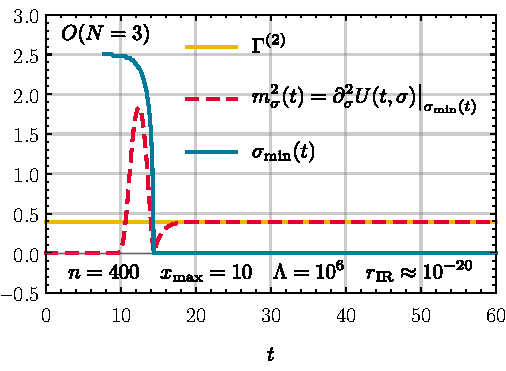
\includegraphics[width=\subcaptionFigureWidth]{0d/figures/sc_i_on_3_n_400_xmax_10_lambda_1e6_tir_60_mass_minimum.pdf} % left figure
		\captionsetup{width=\subcaptionFigureWidth}%
		\caption{%
			The \frg{} flow of the minimum $\sigma_\mathrm{min} ( t )$ ({blue}) of the effective potential $U ( t, \sigma )$ and of the curvature mass $m_\sigma^2 ( t )$ of the \sigmaMode{} ({red-dashed}) evaluated on the equations of motion~\eqref{eq:definition_j_t}, \ie{}, at the flowing minimum.
			The {blue} curve sets in after a unique minimum at $\pm \sigma_\mathrm{min} ( t )$ has formed.
			As \uv{} \ic{} we use \cref{eq:testing_scenario_non-analytic_quadaratic_asymptote}. 
			We used the exponential regulator~\eqref{eq:exponential_regulator} with \uv{} scale $\Lambda = 10^6$.
			The curvature mass $m_\sigma^2 ( t )$ was extracted from $u ( t, \sigma )$ via \cref{eq:derivative_1_forward_error_2} at the moving $\sigma_\mathrm{min} ( t )$.
			The horizontal ({yellow}) line denotes the exact \ir{} result $\Gamma^{(2)}\simeq 0.397$ at $\sigma = 0$, which must agree with $m_\sigma^2$ in the \ir{}, where $\sigma_\mathrm{min} ( t ) = 0$.
			\fromFig{12}{zerod1}%
		}%
		\label{fig:sc_i_on_3_n_400_xmax_10_lambda_1e6_tir_60_mass_minimum}%
	}%
	{\fullWidthTwoColumnFigureSpacing}%
	{%
		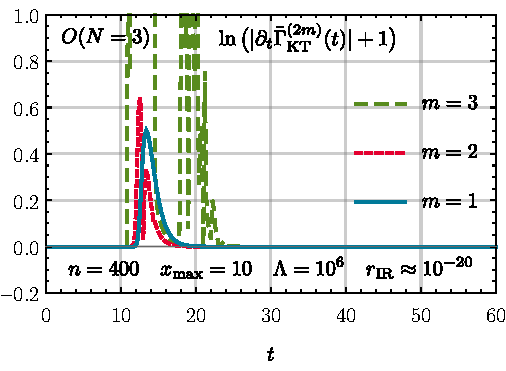
\includegraphics[width=\subcaptionFigureWidth]{0d/figures/sc_i_on_3_n_400_xmax_10_lambda_1e6_tir_60_changing_rates.pdf} % Right figure
		\captionsetup{width=\subcaptionFigureWidth}%
		\caption{
			The rate of change in $t$ of $\bar{\Gamma}^{(2m)} ( t )$ at the \ir{} minimum $\sigma = 0$ for $n = 1, 2, 3$ during the \frg{} flow.
			This rate of change is defined as the numerical \rgtime{} derivative $\partial_t \bar{\Gamma}^{(2m)} ( t )$ over the \rgtime{}.
			$\partial_t \bar{\Gamma}^{(2m)} ( t )$ are calculated via a finite-difference approximation ${[\bar{\Gamma}^{(2m)} (t) - \bar{\Gamma}^{(2m)} (t - \Delta t) ]/\Delta t}$, where $\Delta t = 0.2$.
			$\bar{\Gamma}^{(2m)} ( t )$ are obtained via numerical derivatives \eqref{eq:derivative_1_central_error_2}, \eqref{eq:derivative_3_central_error_2}, and \eqref{eq:derivative_5_central_error_2} of $u (t, \sigma)$ at $x = \sigma = 0$.
			For convenience, we added 1 and took the logarithm to highlight the regions with high rates of change of the observables $\bar{\Gamma}^{(2m)}(t)$ and to identify the freeze-out plateau, where these rates vanish.
			We used the exponential regulator~\eqref{eq:exponential_regulator} with \uv{} scale $\Lambda = 10^6$.
			\fromFig{17}{zerod1}%
		}
		\label{fig:sc_i_on_3_n_400_xmax_10_lambda_1e6_tir_60_changing_rates}
	}
In \cref{fig:sc_i_on_n_400_xmax_10_lambda_1e6_tir_60_flow_errors} (\ie{}, for $N = 1$ and $10$) and independent of the choice of discretization of the numerical derivatives, we observe plateaus for the relative errors for $\Gamma^{(2n)}$ at the beginning and the end of the \frg{} time evolution.
The plateau at small $t$ corresponds to the \uv{} regime and indicates that the \uv{} scale is chosen sufficiently large because no fluctuations are present at the \ir{} physical point until $r(t)$ reaches the scales of the model.
\rgcy{} \eqref{eq:rgcConditionONd0}, hence \uv{}-scale-independence should therefore be fulfilled, as long as we initialize our \frg{} flow at some \rgscale{} which is at the far left of this plateau.
Such a plateau at small $t$ is a sufficient condition for \rgcy{} but not a necessary one, because quantum fluctuations could already work at positions in field space away from the \ir{} physical point and only influence higher-order correlation functions.
We will quantify this in the following.
In the plots various finite-difference stencils with distinct error scaling in $\Delta x$ are used to demonstrate that the plateaus are independent of other sources of errors, like spatial discretization errors\footnote{%
	Incidentally, \cref{fig:sc_i_on_n_400_xmax_10_lambda_1e6_tir_60_flow_errors} also underlines our statement that the spatial discretization errors stemming from the numerical differentiation of $u ( t, \sigma )$ are much more severe than the discretization errors of the \ktScheme{}.
	Otherwise, the curves for the various finite-difference stencils would coincide in the \ir{}.%
}.

For intermediate $t$, we observe strong dynamics and rapid changes in the relative errors for the $\Gamma^{(2n)}$.
The actual values of the relative errors for intermediate $t$ are irrelevant for the current discussion on \uv{} and \ir{} scales.

The plateau at late \rgtimes{} $t$ corresponds to the \ir{} scale of the theory and indicates that the physical observables are frozen and do not change anymore, such that the numerical time integration can be stopped.
As expected, we find that the explicit \ir{} scale strongly depends on the choice of $N$, thus the number of pions and the related strength of advection.
The smaller $N$ and the more diffusive the system, the longer it takes to reach the \ir{}\footnote{%
	This is a well-known observation from all kinds of fluid-dynamical systems.
	It typically takes much longer to reach thermal equilibrium via diffusion alone than when including advective processes.
}: For $N = 10$ the freeze-out already sets in at $t \approx 26$, while for $N = 1$ one has to wait until $t \approx 30$ to find that the dynamics ends.
This is a difference of two orders of magnitude in the \rgscale{}.
In general, our toy model tests indicate that rather small \ir{} scales are needed to actually reach the regime where the observables are frozen. 
Still, for $N = 10$, $r(t \approx 26) \approx 5 \cdot 10^{-6}$, \ie{}, the \ir{} regime begins six orders of magnitude below the model scales.

This observation might also partially translate to higher-dimensional models, meaning that commonly used \ir{} cutoffs might be systematically chosen too large, such that predictive power is lost. Nevertheless, we expect this problem to be the less severe the higher the space-time dimensionality of a model under consideration, because of the larger phase-space (momentum suppression).
The smaller the space-time dimension of a model, the more important are long-range interactions \dash{} quantum fluctuations at small \rgscales{} $k$ \dash{} for the macroscopic observables, which is of course most extreme for $d = 0$.

Furthermore, we observe from \cref{fig:sc_i_on_3_n_400_xmax_10_lambda_1e6_tir_60_mass_minimum} as well as \cref{fig:sc_i_on_n_400_xmax_10_lambda_1e6_tir_60_flow_errors} that the freeze-out scale is slightly different for different observables, because higher \ipi{} \nptFunctions{} seem to be more sensitive to tiny changes in $u ( t, \sigma )$.
In particular, we observe from \cref{fig:sc_i_on_3_n_400_xmax_10_lambda_1e6_tir_60_mass_minimum} that the minimum $\sigma_\mathrm{min}$ is already frozen at $t \approx 14$, while the curvature mass $m_\sigma^2$ still changes drastically after $t \approx 14$ over several orders of magnitude in \rgscale{}.
This is especially interesting for higher-dimensional models: Oftentimes the freeze-out of the minimum is considered a suitable \ir{} scale to stop the \frg{} flow, which is definitely not justified, since the derivatives of the potential \dash{} the curvature mass \dash{} at the physical point are usually still changing.
Using the changing rates of the curvature mass instead of the position of the minimum as a monitor for the dynamic range \dash{} viable numerical \ir{} cutoffs \dash{} has proven crucial in the \frg{} study~\cite{Stoll:2021ori} of the \gnym{} in \cref{sec:gnyFiniteN}.

\halfWidthFigure%
	{0d/figures/sc_i_on_3_n_400_xmax_10_rir_10e-20_cutoff_test.pdf}
	[]
	{%
		The relative error for $\Gamma^{(2m)}$ for $m = 1, 2, 3$ from the \kt{} scheme as a function of the \uv{} scale scale $\Lambda$ for the initial potential \eqref{eq:testing_scenario_non-analytic_quadaratic_asymptote}.
		We use the exponential regulator~\eqref{eq:exponential_regulator} and keep the \ir{} cutoff scale constant at $r ( t_\mathrm{IR} ) = 10^{-20}$.
		Furthermore, for all data points the computational grid size is fixed at $\sigma_\mathrm{max} = x_\mathrm{max} = 10$ and the number of volume cells is set to $n = 400$.
		$\Gamma^{(2m)}$ are calculated from $u ( t_\mathrm{IR} = 60, \sigma )$ via the approximations \eqref{eq:derivative_1_central_error_2}, \eqref{eq:derivative_3_central_error_2}, and \eqref{eq:derivative_5_central_error_2} for the numerical derivatives. The yellow straight line $\propto\Lambda^{-1}$ is for optical guidance.
		\fromFig{16}{zerod1}
	}%
	{fig:sc_i_on_3_n_400_xmax_10_rir_10e-20_cutoff_test}
Next, we explicitly quantify the relative errors of $\Gamma^{(2n)}$, which stem from too small \uv{} scales $\Lambda$ and the violation of \rgcy{} \eqref{eq:rgcConditionONd0}.
To this end, we plot the relative errors \eqref{eq:relative_errors_gamma_2n} as a function of the \uv{} scale $\Lambda$, while keeping the \ir{} cutoff scale fixed at extremely small $r ( t_\mathrm{IR}) = 10^{-20}$.
In \cref{fig:sc_i_on_3_n_400_xmax_10_rir_10e-20_cutoff_test} we observe that the \ir{} observables become independent of $\Lambda$ at rather large $\Lambda \approx 10^6$.
This is several orders of magnitude above the model scales, contrary to what is often used in \frg{} studies in higher dimensions.
If the \uv{} scale is chosen too small, we find that the relative errors of $\Gamma^{(2n)}$ grow proportional to $\frac{1}{\Lambda}$, as estimated in \cref{eq:error_scaling_uv_cutoff}.
Surprisingly, it turns out that the \rgcy{} condition \eqref{eq:rgcConditionONd0} is already violated at rather large \uv{} scale scales $\Lambda \approx 10^5$ and is only fulfilled for $\Lambda \smallergtrsim 10^5$. 
We conclude that great care is required when specifying the \uv{} scale in a \frg{} calculation.

Before we close this discussion, we provide a natural measure to estimate the correct \uv{} and \ir{} scales of a model or theory, even if there are no exact reference values for observables that can be used for comparison with the \frg{} results.
To this end, we plot in \cref{fig:sc_i_on_3_n_400_xmax_10_lambda_1e6_tir_60_changing_rates} the shifted logarithm of the changing rates of the $\bar{\Gamma}^{(2n)} ( t )$ at the \ir{} minimum $\sigma = 0$ over \rgtime{} $t$.
These quantities have to vanish in the \uv{} and the \ir{}, when the relative errors \eqref{eq:relative_errors_gamma_2n} are not changing.

A similar investigation can be done for any other model or theory and can be used as an indication to ensure sufficiently large \uv{} and sufficiently small \ir{} cutoffs: A first estimate may be obtained by choosing $\Lambda$ and $t_\mathrm{IR}$ in a way that the plateaus (or scaling regimes) in figures similar to \cref{fig:sc_i_on_3_n_400_xmax_10_lambda_1e6_tir_60_changing_rates} are of approximately equal \rgtime{} duration than the time interval in which the actual dynamics takes place. 
In the absence of an explicit and accessible error estimate, rates of change are a cheap and simple tool to study the \uv{} and \ir{} limits of \rgtime{} evolution, \cf{} \cref{subsec:gnyFiniteNresults}.